\documentclass[../main.tex]{subfiles}

\graphicspath{{../image/}{../figure/}}

\begin{document}

\chapter{概率}\label{chapter:ch02-概率}

几乎所有机器学习应用场景，都需要处理不确定性。例如，区分皮肤病变是良性还是恶性的图像分类系统，在实际中不可能万无一失。不确定性可以分为两种。第一种是认知不确定性（epistemic uncertainty），也称系统不确定性（systematic uncertainty）。这种不确定性源自有限的数据集大小。随着观测数据的增多，例如更多良性和恶性皮肤病变图像样本，系统可以更好地预测新样本的类别。然而，即使数据集无限大，也仍然无法达到完美的准确率，因为存在第二种不确定性——偶然不确定性（aleatoric uncertainty），也称内在（intrinsic）不确定性或随机（stochastic）不确定性，有时简称噪声（noise）。一般来说，噪声源自人们只能观察到关于世界的部分信息。因此，一种从源头减小这种不确定性的方法是收集不同类型的数据。\cref{figure:ch02-不确定性示例}用扩展到二维的正弦曲线为例说明了这个问题（参见\cref{section:ch01-一个教学示例}）。

\begin{definition}[认知不确定性与偶然不确定性]\label{definition:ch02-两类不确定性}
设某学习系统由规模为 $N$ 的数据集训练得到，其预测结果所携带的不确定性可以划分为两类。若这种不确定性源自数据集的规模有限，即随着观测数据的增多（$N$ 增大）它可以被减小，则称之为\textbf{认知不确定性}（epistemic uncertainty），也称系统不确定性（systematic uncertainty）。若这种不确定性即使 $N\to\infty$ 也不会消失，而源自人们只能观测到关于世界的部分信息，则称之为\textbf{偶然不确定性}（aleatoric uncertainty），也称内在（intrinsic）不确定性或随机（stochastic）不确定性，有时简称噪声（noise）。
\end{definition}

\begin{figure}[htbp]
  \centering
  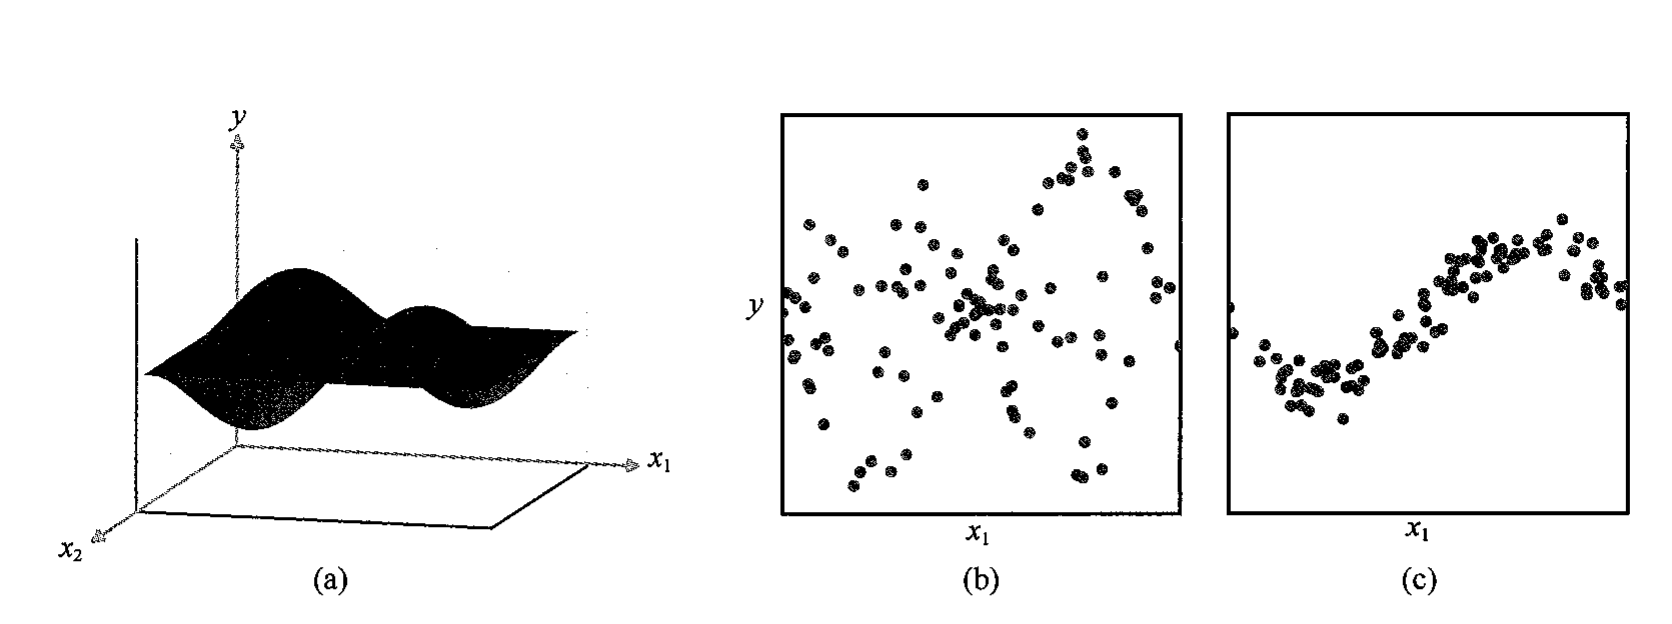
\includegraphics[width=0.95\textwidth]{ch02-fig2-1-sin-regression.png}
  \caption{扩展到二维的简单正弦曲线回归问题。(a) 函数 $y(x_1,x_2)=\sin(2\pi x_1)\sin(2\pi x_2)$ 的曲线图。数据是通过选择 $x_1$ 和 $x_2$ 并计算对应的 $y(x_1,x_2)$ 值，然后加上 Gauss 噪声得到的。(b) $100$ 个数据点的图示，其中 $x_2$ 未被观测到，显示出了较高的噪声水平。(c) $100$ 个数据点的图示，其中 $x_2$ 固定为 $\pi/2$，旨在模拟能够同时观测到 $x_2$ 和 $x_1$ 时的效果，显示出了明显较低的噪声水平。}
  \label{figure:ch02-不确定性示例}
\end{figure}

% SUPPLEMENT: parent=definition:ch02-两类不确定性; kind=motivation; location=紧随其后的 remark（重构新增）
\begin{remark}（重构新增）
这一区分的作用是给“不确定性还能不能继续减小”提供一个判据，而不是给不确定性贴标签。\cref{figure:ch02-不确定性示例}正说明了这一点：图 (b) 只观测到 $x_1$、$x_2$ 被边缘化掉，因而数据点散布很宽；图 (c) 把 $x_2$ 固定为 $\pi/2$ 之后，散布明显收窄。两者之间的差别属于认知不确定性，只要补测 $x_2$ 就能消除；而即使补充再多同一水平的数据，图 (c) 中的数据点仍然围绕曲线 $y(x_1,\pi/2)$ 波动，这一部分波动无法通过增加样本消除，属于偶然不确定性。

条件“$N$ 增大可减小”是判别认知不确定性的关键：它要求不确定性来自对总体分布的估计不足，而不是来自总体的内在随机性。反过来，若一个量的不确定性与数据量无关（例如同一患者重复测量的生理波动），那么无论怎样扩大数据集都不会改善，只能通过引入新的观测变量（也就是本节所说的“收集不同类型的数据”）来缓解。
\end{remark}

在实际的例子中，皮肤病变的活检样本比图像本身的信息量要大得多，这有可能极大提升判断新恶性病变的准确性。如果同时考虑图像和活检数据，则不确定性可能非常小，而通过进一步收集较大的训练数据集，我们或许能将系统不确定性降到一个较低的水平，从而以较高的准确率来预测病变类别。

这两种不确定性都可以用概率论（probability theory）的框架来处理，它为不确定性的量化和操作提供了统一的范式，因此成为机器学习的核心之一。概率可以由两个简单的公式控制（参见\cref{section:ch02-概率法则}），即加和法则（sum rule）和乘积法则（product rule）。结合决策论（decision theory）（参见\cref{section:ch05-决策理论}），这些规则理论上允许我们在给定的已知信息上做出最优预测——尽管我们获得的信息可能是不完整的或模糊的。

概率通常根据可重复事件的频率引入。以\cref{figure:ch02-弯曲硬币}中的弯曲硬币为例，假设该硬币的形状如此，并被多次抛掷，则落地时有 $60\%$ 的可能性凹面朝上，有 $40\%$ 的可能性凸面朝上。因此我们说，弯曲硬币落地时凹面朝上的概率是 $0.6$ 或 $60\%$。严格来说，这时的概率是在无限次“试验”或抛掷硬币的极限情况下得出的。因为硬币要么凹面朝上，要么凸面朝上，所以这两种情况的概率加和为 $100\%$ 或 $1.0$。根据可重复事件的频率来定义概率，是频率学派（frequentist）视角下统计学的基础。

\begin{figure}[htbp]
  \centering
  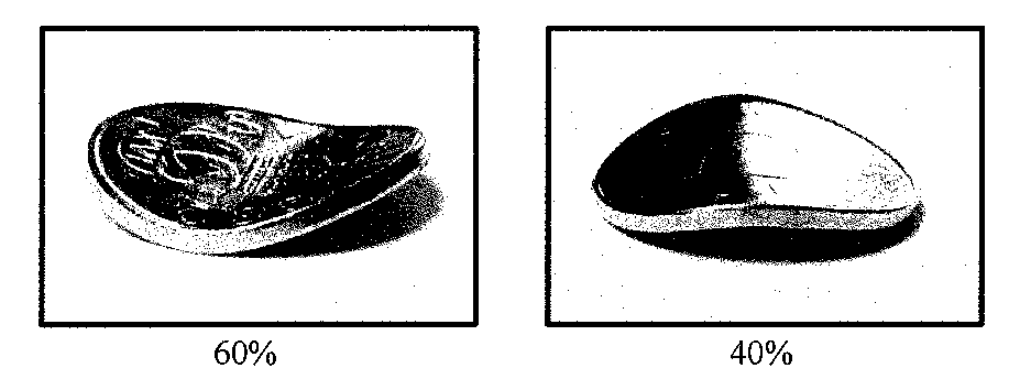
\includegraphics[width=0.62\textwidth]{ch02-fig2-2-bent-coin.png}
  \caption{概率既可以视为与可重复事件相关的频率，也可以视为对不确定性的量化。这里用弯曲的硬币抛掷后落地的情况来说明这两者之间的区别。}
  \label{figure:ch02-弯曲硬币}
\end{figure}

现在假设即使我们知道硬币落地时凹面朝上的概率是 $0.6$，但我们不允许看硬币，也不知道哪一面是正面、哪一面是反面。此时如果让我们猜一下硬币抛掷后落地时正面朝上还是反面朝上，那么硬币的对称性指示我们的猜测应该基于看到正面的概率是 $0.5$。更细致的分析表明，在没有任何附加信息的情况下，这的确是一个理性的选择。在这里，我们使用的是更一般意义上的概率，而不仅仅是事件发生的频率。定义硬币的凸面是正面还是反面，本身并不是一个可重复的事件，它是未知的。使用概率对不确定性进行量化是 Bayes 学派（Bayesian）的观点（参见\cref{section:ch02-Bayes概率}）。这一观点更普遍，而频率学派的概率只是这一观点下的一种特殊情况。如果可以获知一系列抛掷硬币的结果，我们就可以通过 Bayes 推理知道硬币的哪一面是正面（见\cref{exercise:ch02-40}）。观测到的结果越多，我们关于硬币哪一面朝上的不确定性就越低。

\begin{definition}[概率的频率学派解释与 Bayes 学派解释]\label{definition:ch02-概率的两种解释}
称一个事件是\textbf{可重复的}，若它能在相同的条件下被反复试验。把可重复事件 $E$ 在 $n$ 次试验中出现的次数记为 $n_E$。若极限 $\lim_{n\to\infty} n_E/n$ 存在，则把它定义为 $E$ 的\textbf{概率}；以这种“长期频率”的方式解释概率的立场称为\textbf{频率学派}（frequentist）观点。与之相对，把概率解释为对命题成立这一事件的不确定性程度的量化、从而允许对不可重复的命题赋予概率的立场，称为 \textbf{Bayes 学派}（Bayesian）观点。
\end{definition}

% SUPPLEMENT: parent=definition:ch02-概率的两种解释; kind=motivation; location=紧随其后的 remark（重构新增）
\begin{remark}（重构新增）
两种解释的差别不在于公式，而在于“概率从何而来”。频率学派的定义依赖极限 $\lim_{n\to\infty}n_E/n$ 的存在，因此必须先有一个可重复的试验机制；\cref{figure:ch02-弯曲硬币}的硬币满足这个条件，$60\%$ 与 $40\%$ 是抛掷次数趋于无穷时的比值。Bayes 学派则把这个极限当作特例：当命题确实对应可重复事件时，先验信息足够弱，后验概率会收敛到频率，二者一致；当命题不可重复（“这枚硬币的凸面是正面”）时，频率定义失效，而“用概率量化不确定性”仍然有意义。

需要强调的是，Bayes 观点并不与频率观点矛盾，它只是在更大的范围里给概率指派含义；这也是本书后文（例如\cref{section:ch02-Bayes概率}）反复使用的立场。条件“$n_E/n$ 的极限存在”在频率解释中不可省：若试验条件每次都在变化，长期频率可能不存在，此时只能采用 Bayes 解释。
\end{remark}

在非正式地介绍完概率的概念之后，我们现在要对概率进行更详细的探讨，并讨论如何定量地使用概率。本章接下来的内容所阐述的概念将构成本书所讨论的许多其他主题的核心基础。

\subfile{Chapter-02/section-01.tex}
\subfile{Chapter-02/section-02.tex}
\subfile{Chapter-02/section-03.tex}
\subfile{Chapter-02/section-04.tex}
\subfile{Chapter-02/section-05.tex}
\subfile{Chapter-02/section-06.tex}
\subfile{Chapter-02/section-07.tex}

\end{document}
